\begin{abcliste}
\abc The water can rise and fall freely at the wall; it is only stopped sideways. For the wave, the wall is a free end: the crest is reflected upright, and at the wall the incoming and the reflected crest are there at the same time and add up:
\begin{align}
 \ssc{h}{wall} &= \hmF = 2\times\hw = \result{\hmP{0}{2}}
\end{align}

\abc At the wall the water rises once to twice the height of the crest and falls back again: a single bump of height \hmP{0}{2}, as long as the crest takes to pass. (Only a fixed end would stay at rest; at a free end the reflected crest is not upside down.)
\begin{center}
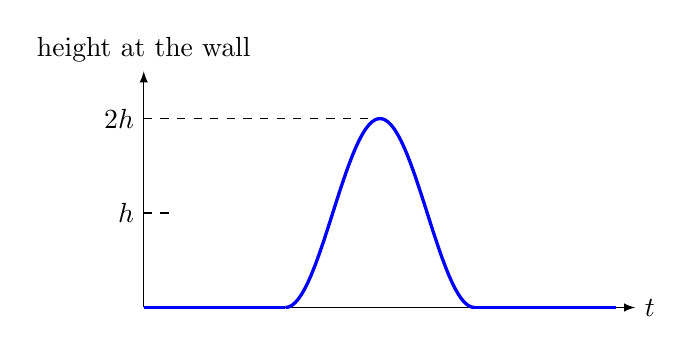
\begin{tikzpicture}[>=latex, x=1.2cm, y=1.2cm]
 \draw[->] (0,0) -- (5.2,0) node[right] {$t$};
 \draw[->] (0,0) -- (0,2.5) node[above] {height at the wall};
 \draw[dashed] (0,2) node[left] {$2h$} -- (2.5,2);
 \draw[dashed] (0,1) node[left] {$h$} -- (0.3,1);
 \draw[very thick, blue] (0,0) -- (1.5,0);
 \draw[very thick, blue, domain=1.5:3.5, samples=60] plot (\x, {2*sin(deg(pi*(\x-1.5)/2))^2});
 \draw[very thick, blue] (3.5,0) -- (5,0);
\end{tikzpicture}
\end{center}
That is why spray shoots up at harbour walls and cliffs.
\end{abcliste}
